%%%%%%%%%%%%%%%%%%%%%%%%%%%%%% -*- Mode: Latex -*- %%%%%%%%%%%%%%%%%%%%%%%%%%%%
%% uhtest-body.tex -- 
%% Author          : Robert Brewer
%% Created On      : Fri Oct  2 16:30:37 1998
%% Last Modified By: Robert Brewer
%% Last Modified On: Mon Oct  5 16:01:29 1998
%% RCS: $Id: uhtest-body.tex,v 1.1 1998/10/06 02:07:14 rbrewer Exp $
%%%%%%%%%%%%%%%%%%%%%%%%%%%%%%%%%%%%%%%%%%%%%%%%%%%%%%%%%%%%%%%%%%%%%%%%%%%%%%
%%   Copyright (C) 1998 Robert Brewer
%%%%%%%%%%%%%%%%%%%%%%%%%%%%%%%%%%%%%%%%%%%%%%%%%%%%%%%%%%%%%%%%%%%%%%%%%%%%%%%
%% 


\chapter{Introduction}

Long duration space flights induce loss of muscle and bone mass. To capture such changes, body composition measures are traditionally measured through Dual-energy X-ray absorptiometry (DXA); however, this is not as feasible in space because of both the high voltage involved and the fluid redistribution which is not captured by current dxa methods \cite{sibonga2015evaluating}. 3D optical (3DO) imaging has been demonstrated to be able to capture body composition as well as DXA, while also being hypothesized to be more easily deployable in space because of its low power consumption, higher mobility, and attunement for accuracy. We have terrestrial models and the main goal of this long-term study is to demonstrate the feasibility of our system to capture body composition in in microgravity situations such as in a parabolic flight. For my thesis, I demonstrate how I built such a system that can be used in such environments. 
\section{Ways of getting body composition}
DXA is commonly used to measure bone density by measuring the absorption of soft tissue and bone using dual X-rays \cite{albanese2003clinical}. The radiation used is considered comparable to one day from background radiation at sea level; however, it should still be minimized in usage \cite{damilakis2010radiation}. Due to its versatility, DXA can also be used for total body composition and fat content measurement.

Body composition comprises of fat, bone, water, and muscle percentage. The four compartment model is shown below \cite{fuller1992four}:
\begin{equation}
	\frac{1}{D_b} = \frac{w}{D_w} + \frac{f}{D_f} + \frac{p}{D_p} + \frac{m}{D_m}
\end{equation}
Db: overall body density, w: proportion of water, f: proportion of fat, p:proportion of protein, m: proportion of mineral, Dw: density of water, Df: density of fat, Dp: density of protein, Dm: density of mineral

Bio-electrical impedance (BIA) is used to measure volume, shape, or tissue electrical properties using the general formula \cite{jaffrin2008body}:
\begin{equation}
	Z = \frac{\rho L}{A}
\end{equation}
$\rho$ is the resistance which is a metric of the tissue. L is the distance between the electrodes placed on the body. A is the area. Z is the impedance. By placing a source and sense electrode on the person's hand and foot and sending a current through the body one can measure the voltage and current with respect to time on each electrode and can determine body water and subsequently body fat \cite{khalil2014theory}. Fat and bone have higher resistance than fluid and electrolytes and thus the electrons travel differently through these mediums.

Underwater hydrostatic weighing is also used to determine body fat to lean mass ratios based off of Archimede's Principle of displacement taking advantage of the constant density of fat mass and fat-free mass.

In this work, I concentrate on using imaging which has certain advantages including being non-invasive and relatively inexpensive, along with being portable.
\section{Sensor Types}
In regards to the sensors two main types were considered, stereo cameras and time of flight (ToF). The ideal imaging equipment roots its foundation on the attunement to the capture and reconstruction of precise depth measurements. Some basic requirements include the sensor to be lightweight because it needs to be mounted. It must also have good general properties involving frame rate, resolution, precision of
acquisition, and field of view. The ideal specifications surround image quality and noise. Basic hardware feature that directly affects image quality as such are pixel size and depth reconstruction algorithms. For depth, there
are a few important things: the Z-accuracy, which is the depth data accuracy, the fill rate which
evaluates the percentage of the depth coverage of the image, the Root Mean Squared Error (RMSE) which evaluates the
spatial noise or spatial depth uniformity. And the temporal noise which evaluates the temporal
uniformity over sequential frames. Other traits between sensors are mostly comparable and
company provided specs are reliable.

ToF is fast and the depth reconstruction does not face the same problems that stereovision faces such as matching up two image planes, but it usually suffers due to this in resolution, because they are more susceptible to light. ToF uses the phase shift of amplitude modulated waves to measure distance, while stereo takes two pictures of the scene at different positions and generally uses epipolar geometry or more recently deep learning. The depth depends on the reconstruction algorithm. Intel camera also have an optional infra-red used for feature matching in low contrast settings. One such way of calculating the depth from time of flight is based on a simplified ideal model.

\begin{equation}
	d = \frac{c * \varphi}{4\pi * f}
\end{equation}


\begin{equation}
c = \lambda * f
\end{equation}
c is the speed of light in meters per second, $\lambda$ is the wavelength and f is the frequency in Hz.
\begin{equation}
	\varphi = ArcTan(\frac{A_1 - A_3}{A_2 - A_4})
\end{equation}
A represents the amplitudes of the received signals at four equally spaced intervals.  $\varphi$ gives us the phase shift.

For stereovision, usually several pre-processing steps are done. After which, epipolar geometry is often used. A point on the image plane of one sensor which is converted from 3D to 2D, through perspective projection, is somewhere in the image plane of the other sensor along the epipolar line. Using a criterion, we choose from several candidates of that line. In this manner, we can understand the utility of the infra-red pattern projection. Using geometry, one can then obtain the depth values as the intrinsic and extrinsic camera parameters are known \cite{ayache1988rectification}. In general ToF technology is more expensive than stereo and is slightly larger. ToF is more useful in cases which have significant motion such as drones and autonomous vehicles. Stereovision is also sensitive to color unlike time of flight because color information is used in the depth algorithms. In some cases color information may be useful such as for a neural network. As such it is not as robust to weather conditions, low lighting, and the range is shorter than ToF. The main plus though is the resolution and field of view are better for stereovision than time of flight at the same price point, along with more commercial sensors using stereovision and thus more software integrated with stereovision sensors.
\section{Overall Philosophy}
"Garbage in garbage out". To obtain accurate output requires informative input. Then it's a matter of creating a function that maps these values whilst minimizing error. A primary such first choice of action is determining the inputs. What format should the inputs be in? We must limit ourselves to some relatively finite input such as images. So these images contain values from sensors. And these sensors can be your normal camera or time of flight. Other input may include descriptive information such as categorical variables like demographics: race, gender, age, etc. There are different ways to use and combine these.

This work concentrates on utilizing depth data from sensors for 3D reconstruction. It is possible to go directly from the depth data to body composition without the need for feature engineering such as mesh reconstruction, caesar point placement, templating, principal component analysis, and linear regression to get to body composition and shape. The primary reasoning for feature engineering is to get performance more quickly off the bat and in cases where one does not have vast amounts of data such as in the millions of examples which deep learning could more effectively utilize.

This thesis is composed of several main parts. The first is the comparison of the sensors for data collection. The second is the modeling of the data. The third is data simulation, augmentation, and validation through means of distribution approximation methods such as microgravity environments. Finally, the preparation for data acquisition in one such special environments known as parabolic flights.
\section{File Formats}
Here I describe a few file formats that are in use for further clarity of this document. First is the wavefront obj file which is for point cloud data. Second is the polygon ply file which is also for point cloud data but has additional functionality such as color information. Third is the pp file which is point placement data for the caesar dataset used in meshlab known as picked points. Fourth is image data which pngs are primarily used in this project. Fifth is depth data which can also be stored in pngs. Starting with image data which most people are familiar with, a color image will often have 3 channels one for red, one for green, and one for blue. An image that is 720 x 480 for example is 720 pixels wide and 480 pixels high. An image will contain 720 x 480 x 3 values. Depending on the acquisition format, there may be a limit to the lower and upper bounds of these values. Commonly it is a byte, 8 bits, so from 0-255. Depth data on the other hand only has one channel usually. And the upper bound of the value is usually limited by the data type used such as a 64 bit structure. It will often represent the distance from the sensor to that point in meters.

The obj file is a human readable format shown in figure 1.1. It contains information for the position of each vertex, the UV position (texture mapping axes) of texture coordinates, vertex normals, and faces. Vertices are listed in counter-clockwise order. A vertex is represented as v x y z. Vertex normals are optional because faces define them. They are represented as vn x y z. Optionally, one can specify textures with vt u v. Generally a face will be defined as f v1 v2 v3. The one main requirement for an obj is the vertices. When opening this in a viewer, one can see the points. Many computer graphics, 3D printing and game rendering engines also require the face information to connect the dots along with texture information for how the faces look. In this project, only vertices and face information is used.
\begin{figure}[!htb]
	\caption{Obj File Example}
	\centering
	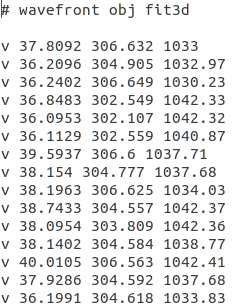
\includegraphics[width=0.25\textwidth]{images/obj_file.png}
\end{figure}
\
The ply file shown in figure 1.2 is similar to the obj file. There is also the option for encoding and compression of this file; otherwise, the file is human readable like the obj file. A plus over the obj file is the ease of adding color information. There is the list of vertices and faces and when one wants to add color to a face one can specify a tuple such as (r, g, b) to represent the red green blue values for that face. For plyfiles, there is an off the shelf library but I did not find a convenient one for objs and so made my own. 

\begin{figure}[!htb]
	\caption{Ply File Example}
	\centering
	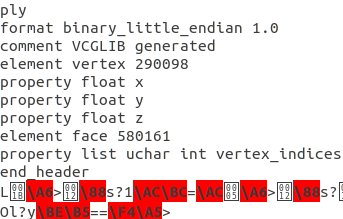
\includegraphics[width=0.3\textwidth]{images/ply_file.png}
\end{figure}
\begin{figure}[!htb]
	\caption{PP File Example}
	\centering
	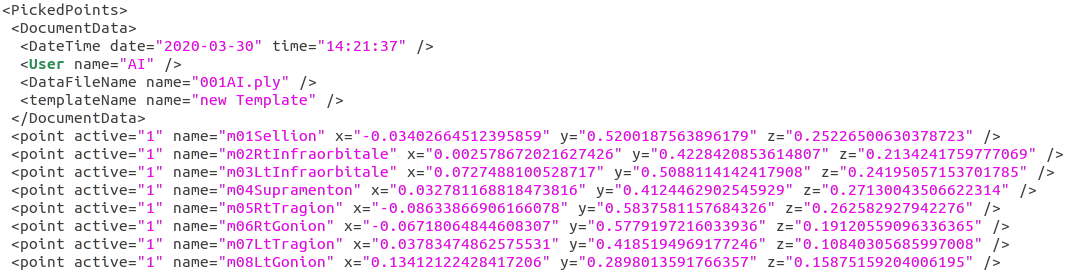
\includegraphics[width=1.1\textwidth]{images/pp_file.png}
\end{figure}

The PP file shown in figure 1.3 is essentially an XML format with a few components \cite{bray2000extensible}. The PickedPoints class is shown in figure 1.3, the document data which can contain some optional information such as : time, username, filename, and template name are linked underneath. Next it includes the 75 landmarks which x, y, and z coordinates, along with the anatomical name of that point \cite{robinette2002civilian}.

\section{Caesar Dataset}
The Caesar dataset (Civilian American and European Surface Anthropometry Resource) was a project by SAE whence they collected data on 2400 US and Canadians and 2000 Europeans. It includes 75 landmarks, 3D model scans, and traditional 1d measurements done with a tape measure and caliper. They include demographic information of their participants who range from ages 18-65. The 75 landmarks which I try to automatically find include points such as the sellion, iliocristale, metacarpal-phalangeal, dactlyion, tip of the nose, and so forth across the entire body. Why this is done is because they thought these points are indicative of key features of people which can provide pertinent information for use in various algorithms such as deforming a template mesh to a scanned mesh.

\chapter{Previous Work}
I start off by showing a variety of 3D scanning machines in figure 2.1. They use kinects and intel sensors. Kinects are time of flight and intel utilize traditional stereovision.
These scanners are all good and use a variety of kinect sensors and intel sensors, but are rather inflexible in serving the purpose of imaging in microgravity situations. As such, I built my own system for this. Also, the software for these systems is not open source and depends heavily on the precise geometry of these systems which can be costly. It is important to note the differentiation between these 3D optical scanners and other 3D imaging methods such as CT scans.

\begin{figure}[!htb]
	\caption{Sizestream (SS20), Naked Labs(S/N PVT0000418260023), Fit3D(ProScanner 4.0 S/N10007730), and Styku Scanners(S/N 085570340147)}
	\centering
	\includegraphics[width=1\textwidth]{images/scanners.png}
\end{figure}

\section{Depth Imaging and 3D Reconstruction}

Next I briefly summarize a fundamental work on 3D imaging \cite{izadi2011kinectfusion}. KinectFusion was a seminal work in which Microsoft developed a time of flight sensor and developed algorithms for real time reconstruction of a scene. Their method comprises of four main parts. Part one is the surface measurement, which includes the raw depth measurements along with a dense vertex map and a normal pyramid map being generated. Part two is the sensor pose estimation which is done by predicting what the surface should be like from the previous data and using multi-scale iterative closest points to the current data. Part three is updating the reconstruction by fusing the current measurement with the scene model which is maintained with a truncated signed distance function. The final part is predicting the surface from part three which feeds back into part two.
Further information and a review of state of the art methods is discussed by Xian-Feng Han, et. al. 2019 \cite{DBLP:journals/corr/abs-1906-06543}.

In 2005, Brett Allen wrote his phd thesis on learning body shape models from real-world data \cite{allen2005learning}. Both sensor technology and algorithms have come a long way since then. A major dataset came out of an SAE project starting in 1998. This data is not public, however is the first major dataset with anthropometric measurements along with 3D stitched models from scanning of 2400 men and women.

\section{Neural Networks for Point Cloud Data}
One of the seminal deep learning papers on 3D input was PointNet \cite{DBLP:journals/corr/QiSMG16}. It was a method used for classification and part/semantic segmentation. A couple years later, dynamic graph convolutional neural network took this further by using dynamic updates to the graph \cite{DBLP:journals/corr/abs-1801-07829}. While these methods are general, there are also more specific methods for reconstruction. A systematic approach for constructing 3D human models from 2d images was demonstrated by Yueh-Ling Lin, et. al. 2010 \cite{5645897}. The Planck Institute published results on obtaining a mesh from a single 2d image using a combination of their previous conventional method and deep learning \cite{kolotouros2019learning}. The method uses a CNN followed by their previous work SMPL and these use a self improving loop. This was tried briefly in this project. Deformable Shape Completion with Graph Convolutional Autoencoders was considered as the paper shows results on taking in an essentially partial mesh and completing it \cite{litany2018deformable}. 

\section{Sensor Testing}
Several papers have done sensor testing with depth cameras. The overall methodology was studied in these papers which are not discussed here for sake of brevity\cite{sophian2017evaluation} \cite{khoshelham2012accuracy} \cite{langmann2012depth} \cite{sankowski2017estimation}. Techniques such as sensor error, fill rate, spatial noise, and temporal noise are chosen from these.


\section{Landmark Prediction}
I briefly describe some previous related work. In Lu and Wang's work \cite{lu2008automated} they use 3D scanners and first segment the body by using silhouette analysis. Initial searches are done using vertical and horizontal manual estimates. Gray-scale detection is used for the identification of armpits. Following the contour of the human-body they extract more points including the cervix and the bust for a total of twelve landmarks. They validate on 189 subjects. In Semi-Automatic Prediction of Landmarks on Human Models in Varying Poses a Markov Graph Network is used. The graph however is obtained manually. 200 people are used \cite{wuhrer2010semi}. Parametric body shape models were created for standing children aged 3-11 years but not adults \cite{park2015parametric}. Several models take in several depth frame data to create a shape model \cite{deng2019neural}. Lu et al. matches the point clouds, generates a skeleton, and uses iterative linear blend skinning for learning joints \cite{lu20193D}. Stanford developed a similar idea by first registering meshes, then using a graphical model with segmentation with EM to get 15 parts of a human model using the concept of rigid skeleton parts which are transformed across sequences \cite{anguelov2012recovering}.


\chapter{Methods}
There were several things I worked on. The first is a review of different sensor technologies and subsequent testing of the top ones. Next was the development for the Zero G Parabolic Flight which are scheduled for the summer. Third was simulating microgravity and testing them. Fourth was seeing the impact of pose on the resulting steps and final measurements. In no particular order, I start off with a graph neural network.

\section{Graph Neural Network for Automated Body Composition and Anthropometry}
One such deep learning method that is used for 3D data inputs are graph neural networks. The one I used specifically is called dynamic graph convolutional neural network (DGCNN) \cite{DBLP:journals/corr/abs-1801-07829}. It consists of n vertices, each of which are tuple of 3 numbers. In order to apply the convolution operator, one must define an edge. With 2d images, an edge is any pixel that is adjacent to another pixel within the kernel length. For a graph, different distance metrics can be used. DGCNN uses pairwise euclidean distances. The k nearest points are used for the subsequent convolution. Next comes the convolution kernel, which the authors define as
\begin{equation}
	E_{ij} = ReLU(\theta_i * (x_j - x_i) + \theta_j * x_i)
\end{equation}
$\theta$ represents the weights of the networks. Then comes max pooling for all such node j in the neighboring set of node i:
\begin{equation}
F_{ij} = Max(E_{ij})
\end{equation}
Before the point cloud goes into this architecture, they apply a matrix transformation using the coordinates and the differences with their neighbors.
They prove certain desirable properties such as permutation invariance and translation invariance and achieved state of the art results.
While they used their architecture for classification and segmentation, I convert it into regression . In the Caesar dataset, 75 landmarks are manually picked which allows a standardized template of 60k nodes to fit to the original mesh that has several hundred thousand points. Usually this may take several minutes for an expert user and can take up to an hour for a beginner.
A landmark is defined as an (x, y, z) coordinate and there are 225 such numbers that are needed to be predicted in a regression case. The other method is semantic segmentation, in which there will be several hundred thousand points which will each need to be classified into 75 classes, resulting in many predictions. Some of these predictions may not even be exactly precise as the landmarks may not coincide directly with a point. It is hypothesized that training is easier in the beginning; however, in the long term one would expect a degradation in results due to noisy labels. This noise comes from the fact that many points don't belong, and only 75 are really needed. With regression, one can predict the exact point and get to perfect performance, but the beginning of training may be more difficult.
The other method considered was taking in the entire mesh including face information as done by MeshCNN \cite{hanocka2019meshcnn}. It is unclear however as to the utility of face information compared to nearest neighbor information from dgcnn.

Thus for automated body shape analysis a deep learning model was reoriented from DGCNN. 5000 scan were used for this data. Sex, height, weight, BMI, and ethnicity were used as non-image features. I got a basic catboost model with the non-image features. The graph neural network uses 1024 vertices, scaled to a unit sphere and augmented. I saved .obj files into hierarchical data files (h5). 

I performed segmentation which allows for a more pleasing visualization of the resulting mesh. It also helps reduce the output space of the network. This does add complexity to the labels as now each point needs to be labelled where previously only 75 points were labelled. Several options here include having a 76th category which is none of them and considered an "other" label. This is the case where there are let's say 100,000 vertices and with only 75 vertices belonging to a landmark. In the simple case we make the rest of them into the 76th category, which will be 99,925 vertices. It's not clear the best way to label all the points though. Do I just take the closest point to the label and label that point and disregard the rest? I take the simplest approach algorithmically where I label all of the points to which label they are closest to. In some sense, we can compare this to label smoothing where we relax the confidence on the labels to help prevent over-fitting.

\section{3D Reconstruction}
For 3D reconstruction I use methods such as SPIN \cite{kolotouros2019learning} ,Kinect Fusion, and RecFusion. SPIN uses a neural network but weights are not shared publicly and thus requires extra time to train a model. I show my results primarily using RecFusion. RecFusion is used because it has a clean interface and has the best results of the three.
\section{Sensor Comparison}

\subsection{Specs}

I did a review of the sensor technologies out there excluding the commercial systems mentioned in previous works. The sensors that were physically tested are the Intel D435 and D415, the Microsoft Kinect XBOX 360, the Microsoft Kinect for Windows, and the Microsoft Azure Kinect. I looked up their specs such as resolution, depth accuracy, and frame rate. I then benchmarked them on depth accuracy, temporal noise, spatial noise, and fill rate. These benchmarks were also done at varying distances. To do so, I made a simple setup. I used an imaging chart and a laser measure (Bosch Blaze Pro 165' Laser Distance Measure GLM165-40). I used 10 frames for each test.

I reviewed the spec sheets for these sensors including depth formats, resolution, frame rate, operating range, the color sensor, field of view, etc.
Some of the specs are publicly available but they do not list complete information most likely for commercial reasons. It was important to us to do custom testing specific to our application in addition.

To calculate the approximate distance based on the field of view, we can do the following:
\begin{equation}
	Tan(\theta) = \frac{H}{D}
\end{equation}
H is the horizontal distance of capture and D is the depth distance for capture. This was useful for initial calculations for field of view and distance requirements.
\begin{figure}[!htb]
	\caption{Trig}
	\centering
	\includegraphics[width=0.2\textwidth, angle=0]{images/tan.png}
\end{figure}

\subsection{Testing Setup}
I bought an art easel (T-sign B076X3WZHB) to hold the chart, but ended up attaching the chart to the wall shown in figure 3.1 because I couldn't get the easel height to be sufficient for testing purposes. A tripod (Vanguard Alta Pro 263AB) for the camera is used. Initially 480 LED lights 3200-5600K CRI 96+ lights were used however the indoor lighting was sufficient and AC problems did not arise. Lights were to be positioned behind the camera at 45 degrees, with the test chart in front, but it was difficult to prevent shadows during testing because the configuration had to keep changing. 
\begin{figure}[!htb]
	\caption{Sensor Testing Setup}
	\centering
	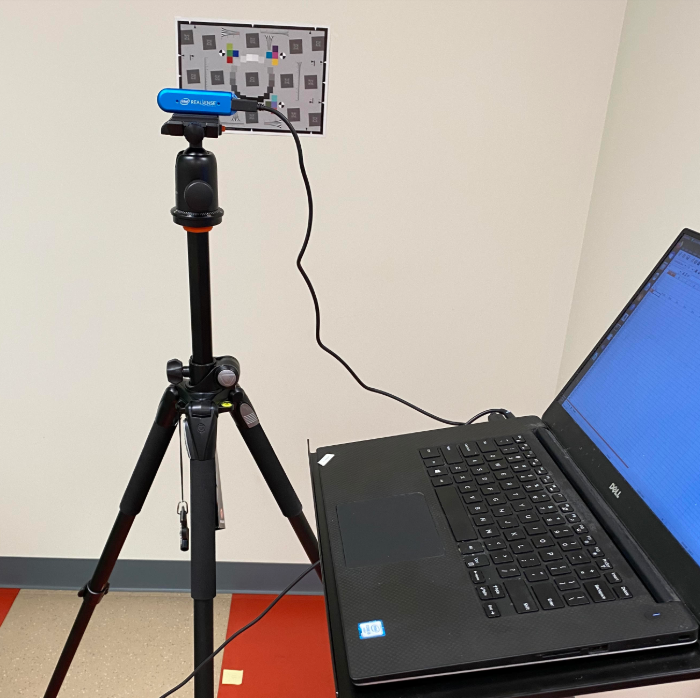
\includegraphics[width=0.4\textwidth, angle=0]{images/sensor_testing.png}
\end{figure}

\subsection{Custom Testing Metrics}

In order to choose the best sensor one could use intermediate metrics that define how good that sensor is or one could use all of those sensors in the overall imaging setup and analysis and see which one works the best. The metrics I used are similar to the report \cite{depthtesting}. Ideally, both should be done. I started with the first as the latter is more time consuming. The metrics thus defined are Z-accuracy, fill rate, spatial noise, and temporal noise. The Z-accuracy says how accurate the depth sensor is in relation to a ground truth (GT). I average the differences in depth sensor values and ground truth across a manually chosen ROI which I kept to be as small as possible around 60 x 60 pixels to minimize color/depth alignment problems. Each metric is for a given single frame and was then averaged across 10 frames. 10 frames were chosen arbitrarily; however, the frames used are after the first 30 frames because the sensors may take some time to warm up and the values in these first frames may be wrong. In equation 3.4, some abbreviated notation is used. The box is the ROI chosen and p includes all pixels that are an element of that box. We take the Image and ground truth (GT) differences and average these.
\begin{equation}
	z \; accuracy = \frac{1}{n}\sum_p(Image - GT) \forall p \in box
\end{equation}
The fill rate relates to how many of the depth pixels are valid. This is useful as some sensors have high accuracy but low fill rate. This is the percentage of pixels that are non-zero.
\begin{equation}
	fill \; rate = \frac{\sum_p[I_p >= 0]}{\vert p \vert} \forall p \in box
\end{equation}
Spatial noise I define as the standard deviation divided by the mean distance.
The RMSE or spatial noise is useful to determine the x-y noise from a plane that is approximately equidistant from the imaging sensor along the lines of sight.
\begin{equation}
	noise = \sqrt{\frac{1}{n-1}\sum_p(I_p-{\bar{I_p}})^2} \forall p \in box
\end{equation}
n is the number of pixels used.
Last comes the temporal noise. Which is essentially the same as spatial noise except we take it across frames of the same pixel location.
\begin{equation}
	temporal \; noise = \sum_p\sqrt{\frac{1}{n-1}\sum_{f=1}^{10}(I_{pf}-\bar{I_p})^2} \forall p \in box
\end{equation}
These 4 metrics are what I test and are defined in the report by Intel \cite{depthtesting}. In addition to that, I compare things such as frame rate, field of view, weight, dimensions, resolution, sdks, minimum z distance and maximum z distance.

\section{Categorical Extreme Gradient Boosting to Predict Body Composition Using Demographic and Anthropometric Information}
I used Catboost \cite{DBLP:journals/corr/DorogushGGKPV17} in order to model body composition using demographic information including sex, height, weight, and ethnicity to get total body fat on the shape up data \cite{article}. As this was a side project, which I only spent a week on, most of it to prepare the data, I only had time to run through the default parameters and do one cross validation experiment. 

\section{Parabolic Flight Setup}
The original plan was to have parabolic flights during the summer of 2020 but when we started looking into dates for Zero-G flights, they had regular flights then but only had research flights during the spring and fall. Thus we chose to attempt to get ready for the spring. It was a bit rushed and we almost made it, ultimately though, the flight was postponed for reasons outside of our control.
To take a 3D imaging system aboard such a flight required certain things. Some systems have a mirror which encases the sensors. This is not necessary in Zero-G as one does not want any object to crack the mirror and the mirror is not needed for imaging. Other scanners such as the Sizestream are extremely heavy and bulky and use many sensors. The height of it is larger than 60 inches which is the maximum height an object can be when brought onto the Zero-G flights. I built my own imaging system and after testing the sensors, I selected the best one.
Figure 3.2 below is what the general setup looks like.
\begin{figure}[!htb]
	\caption{Astro 3D Imaging Setup}
	\centering
	\includegraphics[width=0.3\textwidth, angle=0]{images/mannequin.png}
\end{figure}

The specific maneuver of the aircraft is ascending at \ang{45} followed by a flattening of the plane followed by a \ang{45} nose low fall. The G-ForceOne contains 36 seats and is 60 feet long and 10 feet wide. Due to safety concerns, the maximum height of any equipment is 60 inches. Figures from Zero-G are shown in figure A3 and A4 in the appendix. The aircraft contains attach points that are 20" x 20" (+/-1/16"). Bolt spacers are used with 3/8-24UNF threaded holes along with AN6 steel bolts for securement of equipment. Other requirements included the material to be at least 1/2" thick and 24" x 24" minimum. As such, a wood board was used that is 24" x 24". This was chosen over metal because of the dampening of vibration and for ease of drilling. Straps for carrying and anchoring are used including: CGU-1/B, S0203-0338-B, and 104410P. The power type aboard to be used is 115 volts ac, 60HZ, three phase. The aircraft lighting is at 5600 kelvin and are LEDs suitable for general photography and this type of imaging. On-board tools are properly labeled and to be stored in a toolbox. Before flight, a test readiness review is required.
The specific parts that were used are as follows: 1 inch diameter steel flange for attachment of the pole to the platform. The pole used is metal for the parabolic flight and pvc for adjustable lengths on ground. Screws were used to attached the flange to the platform. Four holes were drilled into the platform for attachment to the plane floor using AN6 steel bolts. A tight plastic cap was attached the top opening of the pole to soften any physical impact. Threaded clamps were used to attach the sensors to the pole at adjustable positions.

\section{Creating The Ideal Imaging Setup On A Plane vs On The Ground}
There are a few differences with the ideal imaging setup on plane vs on ground, one such being timing. Because each parabolic arc is limited to only 8-15 seconds of microgravity, we only could shoot for 8 seconds at max to be safe. While on the ground, time is only a concern due to funding for the subject's time and their availability. Thus when choosing the best parameters on ground, I tested various setups. This included sensor type, frame rate, sensor height, rotation speed, laser power, and minimizing laser interference.
\section{Microgravity Simulation}
Here I discuss the different methods we considered to simulate microgravity on the ground. These included underwater imaging, inversion table, and gravity boots (Teeter EZ-Up Gravity Boots with Adapter Kit) in which the person would hang upside down and would be imaged with the single senor protocol.

\begin{figure}[!htb]
	\caption{Inversion Table}
	\centering
	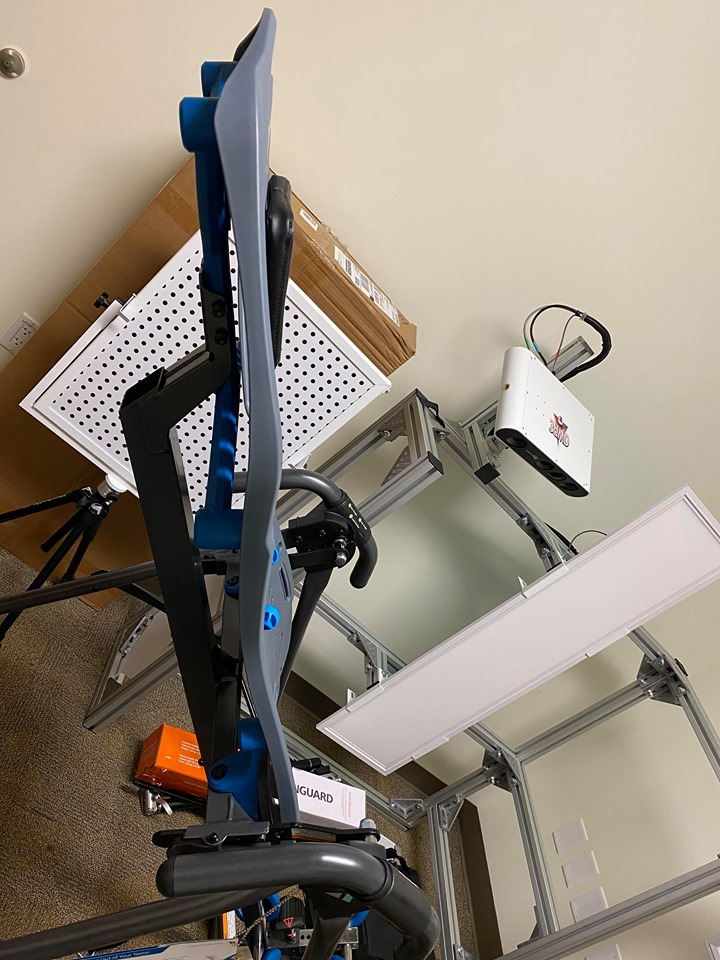
\includegraphics[width=0.4\textwidth]{images/inversion.jpg}
\end{figure}
\subsection{Underwater Imaging}
Planning for underwater imaging was briefly explored. A 2016 paper by Disney research \cite{digumarti2016underwater} used Intel Realsense cameras and a custom capture device. They demonstrated how calibration is different underwater along with the refraction model required. With such results, one could go on to perform 3D reconstruction from this mapping. Some things that have not been done before include a complete scan of human bodies underwater which may require a scanning protocol and/or multiple sensors.
\subsection{Inversion Table}
A sample protocol is described as follows using an inversion table (Teeter FitSpine X1 Inversion Table) shown in figure 3.3. We want to capture different angles from -90 to about -45 degrees. We want to capture at intervals x = 15 degrees. Each subject will be different on the amount of time they can handle. We want to capture 135 / x angles for y amount of minutes. Y is 5 minutes, where 10 minutes is extreme, while some people may only be able to handle a few minutes. How much does it take for a subject to go back to baseline? Let’s say y +- e minutes, where e is close to 0. So to capture one angle will take 10 minutes if it’s 15 degrees, that’s 9 takes, which is about 90 minutes. There are of course different considerations for the angle interval x, and time interval y. The main thing depends on time constraints and subject health. The protocol could be reversed too, to see if the order of inversion has an effect. The inversion table itself is 58” x 29” x 61”. Currently one camera can be attached to the inversion table with a stick and clamp. For inversion table imaging, it would require the single sensor moving protocol. Same goes for gravity boots. 

\section{Mesh Quality}
There are various ways of ranking mesh quality. One such way is using a human to rate the quality. With enough data, one could create a deep learning model. This is quite time consuming. Another method is to run each mesh through different pipelines and see how it performs on the end result for getting values such as body composition. This methodology is also good but our current methodology is not entirely automated. There are many ways of defining similarity. Meshes are similar in the sense that they are numerically represented like images. But they are different because there is no direct correlation between vertices like that of images which are aligned by x-y position. In this case, one can use a neural network and get some intermediate representation and get the similarity from there. Due to time limitations, I perform a simple method for mesh similarity. This method is used in often in the fusion of meshes and/or alignment of meshes. It is known as iterative closest point (icp) in template registration or just euclidean distance generically.

One more well known distance metric worth mentioning is the Hausdorff distance which is a point estimate \cite{huttenlocher1993comparing}:
\begin{equation}
	d_h(X, Y) = max{sup(inf(d(x, y),sup(inf(d(x,y))}, x\in X, y\in Y
\end{equation}
Where sup is supremum and inf is infimum.
Iterative closest points is as follows:
\begin{equation}
	E(R, t) = \frac{1}{N_p}\sum_{i=1}^{N_p}||x_i - Rp_i - t||^2
\end{equation}
$x_i$ and $p_i$ are corresponding points.
While in general, there are many performance things done for this algorithm. t representing translation and R representing rotation. Thus our problem is simplified. On top of this, I perform quadric edge collapse reduction to reduce the search space as a form of sampling \cite{hussain2004efficient}.
The above may be considered as geometric measurements of quality, which do not correlate necessarily with human visual perception. I also try the number of connected components in the graph. A connection between two vertices is defined as a face that includes those two vertices \cite{chung2002connected}.

It is interesting to note many previous works include mesh quality using a reference mesh. Many use the similarity of the surface of the meshes and compare them that way along with visual cues if color is of importance such as contrast. Lastly, I show a ranking correlation between manual and euclidean rankings. The manual ranking involved a manual pairwise sort of the meshes until all pairs of meshes had been visually inspected.
\section{Body Imaging on Babies}
Body imaging on babies is difficult because babies have trouble standing on their own. So typically they are imaged lying down. A result of this is the backside can not get imaged. The method we tried using to get a mesh of babies was a technique called SMIL\cite{hesse2018learning}. After getting it set up we got some preliminary results on fake babies that looked good. The original plan was to see how this could be used for this project too. As there are some cases where the entire body may not be able to be imaged. This includes on an inversion table where the back is once again obscured from view of the sensors regardless of positioning. Another problem is the timing issue on the parabolic flights in which one could stitch together an incomplete view of the person if needed.

\section{Reposing}
One more thing to mention is the use of meshcapade software to repose meshes after they are reconstructed and before data analysis. I use this in the distance calculations for mesh quality to remove positioning problems.
\chapter{Results}
\section{Sensor Testing Results}
For sensor parameters I will list the general parameters used as a base: three sensors, D435, 848 x 480 @ 90 FPS depth resolution, 848 x 480 @ 30 FPS color resolution, max laser power, minimizing laser interference on, live reconstruction on, three feet between the sensors and the object, rotation speed of the turntable of 2.5 RPM, A pose, sensors at heights of 26 inches and 47 inches and 60 inches, lighting on, reconstruction width of 100 and height of 200 and depth of 100, volume resolution of 768 voxels, volume height positioning of -50 and volume width positioning of 10 and volume depth positioning of 100, one rotation, and clothing on. Some of these settings are listed in table A1. A brief summary of the experiment numbers and descriptions is given: 1-12 unclothed mannequin, the rest are clothed. Experiments 13-14 were for depth FPS, 15-16 were for laser interference, 17-21 were for depth FPS again, 22 was with the D415, 23-27 were for rotation speed, 28 was for offline reconstruction, 29-33 were for depth resolution, 34 was with a single moving sensor, 35-39 were for color resolution, 40 was for rotation speed, 41-43 were for a single vertical sensor heights, 44-47 were for 3 vertical sensor heights. In addition, about a hundred scans were taken before this on real humans in an attempt to understand the system, but is not show here because the methodology was not done strictly at the time. 
Figure 4.1 shows the spatial resolution per frame of the D435. This was done to test if the spatial noise changes with the number of frames and the distance. The number of frames does not appear to have an impact; however, the spatial noise is increasing relative to the adjusted distance. This suggests that the closer the sensor to the object the better. There is a limit to how close these sensors can get though.
\begin{figure}[!htb]
	\caption{The Spatial Resolution per frame of the D435 is not affected by the number of frames and the standardized noise increases with increasing distance (in.) between the sensor and chart.}
	\centering
	\includegraphics[width=0.7\textwidth]{images/D435_spatial_resolution.png}
\end{figure}

Figure 4.2 is the chart for sensor accuracy. The average errors in table A3 by sensor in inches are: 0.864 for the D435, 1.366 for the Azure Kinect, 1.739 for the D415, 2.446 for the Kinect Windows, and 2.489 for the Kinect XBOX. While these metrics are not all precise as there is some error from the human, the results shown are averaged across multiple frames to partially counteract this.
\begin{figure}[!htb]
	\caption{The Sensor Accuracy by Distance figure shows the D435 having the lowest error and the Kinects not being able to capture depth well very close up.}
	\centering
	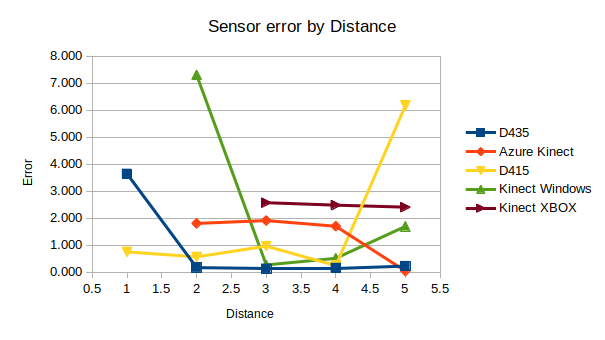
\includegraphics[width=1\textwidth]{images/sensor_accuracy.png}
\end{figure}

For temporal noise shown in figure 4.3, the D415 scored the best in this category. This is partly explained by the D435 being like the D415 except having its sensors more spread out. The winner in this category is the Kinect Azure, then comes the kinect for windows, kinect 360, D415, and D435.
\begin{figure}[!htb]
	\caption{Sensor temporal noise by distance results look similar across the board with the Azure Kinect edging out the competition ever so slightly.}
	\centering
	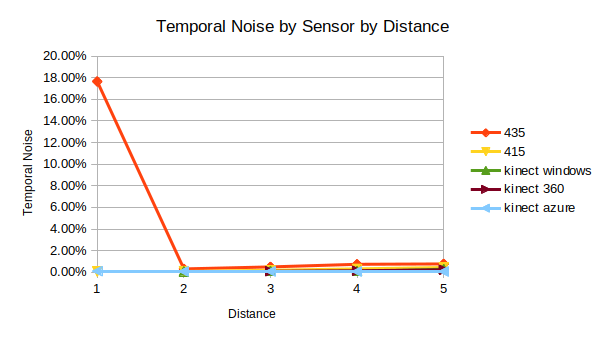
\includegraphics[width=1\textwidth]{images/temporal_noise.png}
\end{figure}

Fill rate shown in figure 4.4, at first may not seem that important but makes reconstruction more difficult when more pixels are missing. If we exclude the Kinect windows because it can't take data at 1 feet away and the Kinect 360 which can't take data closer than 2 feet. The best sensors are D435 at 89.86 percent, D415 at 74.81, then Azure at 70.00.
\begin{figure}[!htb]
	\caption{Fill rate of sensor by distance results weaken the argument for the Azure Kinect.}
	\centering
	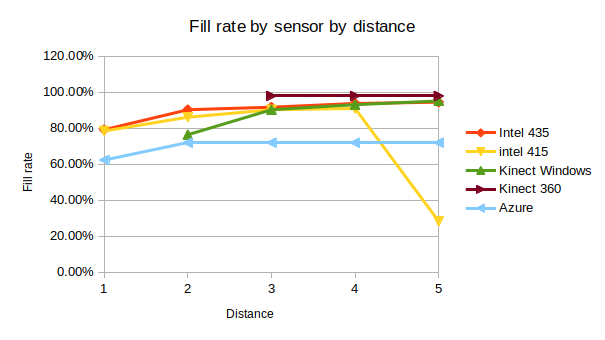
\includegraphics[width=1\textwidth]{images/fill_rate.png}
\end{figure}

\subsection{Sensor Specs}
The D435 is capable of reaching up to 100 frames per second which for this particular imaging application is not that useful, but an application in like drones for example, it could be more useful. One thing to note is that 100 frames per second is a lot especially when combined with multiple sensors and a high quality data connection and cpu is needed to transfer the data fast enough. One can refer to the specs for more details and I just outline some of the main findings. The strong point of the Azure Kinect is its large field of view in certain settings of \ang{120} by \ang{120}. While the D435 has a max depth resolution of 1280 x 720. The depth field of view for the D435 is \ang{85.2} horizontal and \ang{58} vertical. At first it was unclear the advantage this would bring but after testing, I realized the field of view is very useful in allowing the sensor to get closer to the target and allow the target to remain in the field of the view of the sensor. As getting as close as possible is very helpful. The azure Kinect is meant for closer range solutions as the operating range varies between modes but the low end is 0.25m and the high end is 5.46m. Next I do a quick review of the color sensor. It is only in the case of calibration in which the sensor configuration is changing that the color sensor is used to locate the physical calibration boards using color features. When building up the mesh of the scene, it is the depth sensor that is being used and the color sensor has no use, although it could potentially be useful as it provides information unavailable in the depth sensor. There are also sensors that can get distance at much further ranges and these were not considered.


\section{Automated Anthropometry Results}

\begin{figure}[!htb]
	\caption{Training of Automated Caesar Point Placement}
	\centering
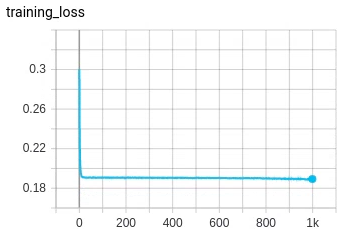
\includegraphics[width=0.5\textwidth]{images/training.png}
\end{figure}
\begin{figure}[!htb]
	\caption{Validation of Automated Caesar Point Placement}
	\centering
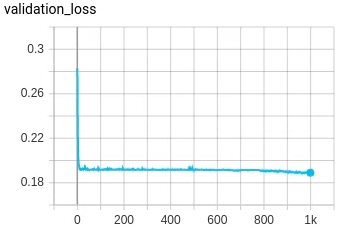
\includegraphics[width=0.5\textwidth]{images/validation.png}
\end{figure}
 \begin{figure}[!htb]
	\caption{Training of Automated Caesar Point Placement without beginning 10 epochs}
	\centering
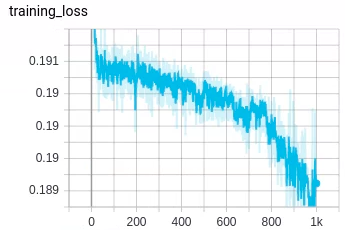
\includegraphics[width=0.5\textwidth]{images/train_close.png}
\end{figure}
\begin{figure}[!htb]
	\caption{Validation of Automated Caesar Point Placement without beginning 10 epochs}
	\centering
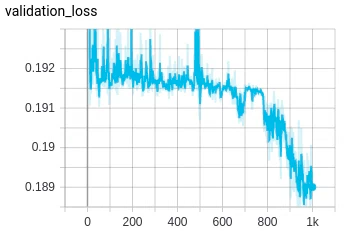
\includegraphics[width=0.5\textwidth]{images/val_close.png}
\end{figure}

We can see the training and validation errors quickly go down after about 10 epochs possibly from simply predicting the mean value of the output in figure 4.5 through 4.8, then continues to go down very slowly. There is no sign of overfitting as the validation loss and training loss are similar to each other. Because only 1024 points are used, this greatly inhibits the capability of the network to learn but was used for quick demonstration purposes. The number does not give me much intuition about the quality of the points. One useful measure would be to see how the final body shape composition results are and the other is to visualize the data. I decide to visualize the data because it could be helpful as a guide for humans if the points aren't placed accurately by the algorithm. Although hyper-parameter tuning would be helpful, it was not the focus of this project. 

\begin{figure}[!htb]
	\caption{Mesh colored by Human labels}
	\centering
	\includegraphics[width=0.5\textwidth]{images/mesh_coloring.png}
\end{figure}

For semantic segmentation, I frame the problem in terms of classification. First I need to label the points. I do this first by taking the closest landmark. An example is shown in figure 4.9. A benefit is preventing overfitting and less training time, the downside is reduced performance. In the end the model struggles to accurately detect landmarks largely in part due to the small training set.

\section{Graph Neural Network and Catboost Body Composition Results}

Some basic data exploration was done like counting of missing data. Distributions of the target variables were plotted, along with the features. Using catboost, after 999 iterations, I got a test RMSE of 2.436kg, std of .791kg, train RMSE of 1.368kg, std of .109kg. It was stated that the best results were 3.070kg for men, and 2.630kg for women using 3D PC + Anthro with 5 fold CV \cite{article}. I also tried a graph neural network. The graph network used 1500 meshes. No transfer learning was done, the model was trained from scratch. Augmentation was done initially for ordering of points, and scaling of points. I removed face information and sampled the vertex information. Next, I reformulated the classification architecture for regression. I did a quick test, trained only on 10 scans, after 50 epochs had about 8000 L1 loss. I also investigated sparse autoencoders, denoising, and contrastive for dimensionality reduction in comparison with principal component analysis.


\begin{figure}[!htb]
	\caption{Random Validation Results of Human labelled vs. Network prediction using classification with 2048 faces}
	\centering
	\includegraphics[width=1\textwidth]{images/label_pred.png}
\end{figure}

I show in figure 4.10 the label's classification front side with point placement in meshlab. Next is the predicted label's classification front side random example with point placement in meshlab.

It's clear the impact of the labelling methodology and the impact on the predictions which are more spread apart than they should be. More results are shown in figures A21 and A22 in the appendix. The main takeaways are the advantages of dimensionality reduction on the mesh for better training results initially, how 76 labels gets worse performance than 75 labels, and the difficulty of regression to predict points on the mesh, requiring a closest points classification to top it off. Even from the error function and visuals, a distribution of differences in coordinates for each landmark could be quite useful.

\section{Parabolic Setup}
The flight was postponed. Several tries were done. Originally a multi-post base was designed. This added support but also complexity. The single pole was quite stable as the weight of the sensors is light.
\section{3D Imaging Testing Results}

\begin{figure}[!htb]
	\caption{Single D435 sensor moving imaging}
	\centering
	\includegraphics[width=0.5\textwidth]{images/dustin_di.png}
\end{figure}

\begin{figure}[!htb]
	\caption{Single D435 sensor moving imaging form fitting}
	\centering
	\includegraphics[width=0.5\textwidth]{images/mw_form.png}
\end{figure}


\begin{figure}[!htb]
	\caption{Mannequin imaged with a laser on and off (experiments 15-16), laser on looks better}
	\centering
	\includegraphics[width=0.2\textwidth]{images/laser.png}
\end{figure}


\begin{figure}[!htb]
	\caption{Mannequin 90fps, 30fps, and 6fps (experiments 17/19/21), at full rotation speed with the fastest rotation speed looking the best although euclidean error did not capture this}
	\centering
	\includegraphics[width=0.5\textwidth]{images/framing.png}
\end{figure}


\begin{figure}[!htb]
	\caption{Mannequin 100, 50, 9 percent speeds (experiments 23/25/27) with lower speeds looking better}
	\centering
	\includegraphics[width=0.5\textwidth]{images/rotation.png}
\end{figure}

\begin{figure}[!htb]
	\caption{Mannequin Depth resolution of 1280x720, 640x480, 480x270 with higher depth resolution looking better}
	\centering
	\includegraphics[width=0.5\textwidth]{images/depth_resolution.png}
\end{figure}

\begin{figure}[!htb]
	\caption{Mannequin imaging with ideal settings for single sensor (experiment 34)}
	\centering
	\includegraphics[width=0.2\textwidth]{images/man_ideal.png}
\end{figure}



We can see in figure 4.14 how at this setting, a higher frame rate helps with the imaging. There is more noise at 6 frames per second and it looks like the background is more part of the body because the sensor has more difficulty tracking the larger change in positioning of the mannequin.

\subsection{Mannequin Imaging}
The best results for imaging come with a single moving sensor. Examples are shown in figures 4.11 and 4.12 and 4.17. As this sensor can capture different parts of the body more easily than when the sensors are static and the object is moving. In general frame rate helps with reconstruction especially when there is more motion of the object. This is the case when our turntable is rotating at maximum speed and it is shown in figure 4.14. On the other hand using automated metrics, this is less clear. It was noticed that minimizing laser interference helped with the reconstruction and it shown on and off in figure 4.13. This happens when multiple sensors emit infra-red and can interact with each other. For the rotation speed of the turntable, slower is better because it makes it easier for tracking of the body. Once again I go based off of visual perception shown in figure 4.15. With depth resolution, higher resolution helps but is interesting to note that this appears to taper off once the resolution reaches 640 x 480 shown in figure 4.16 and is also reflected in the automated error results. The closest 3 horizontal sensors can get to a 6 foot person a turntable is about 3 feet because the calibration pattern needs to be seen consecutively in pairs of rgb sensors. Thus the single moving sensor is able to achieve very nice results by getting a couple feet away. Along with this, there is no need for matching each sensor up to each other, which may give some incorrect results. It is interesting to note the artifacts between the arm and the body and the legs and the body. As the parts spread further apart, the artifacts decrease. For real human imaging, this problem is less of a problem as for the arms, one can use the t-pose which essentially gets rid of all of these problems near the arms. With regards to the lower body, once again, people can split their legs further apart than this mannequin. It is also difficult to maintain the mannequin upright by itself as I spread its limbs further and further apart due to decreased stability. With the discovery of the 3 vertical sensors positioned correctly, the distance gap was able to be closed down to a couple feet resulting in very high quality results.

\section{Mesh Quality Results}
Connected components results are shown in the appendix in figures A18 and A19. In general, it worked as expected. The worst meshes often had many separate islands and the high quality meshes were often well connected. However, there was the case in which a mesh with low resolution was very smooth and was mostly connected resulting in the highest score, but in terms of visual quality, it doesn't look that great. Many have shown the connection before between a difficulty in creating a score that is always correlated with visual quality. However, this may not be that important as its not totally clear to the correlation between visual quality of a mesh by a human and the final performance of a model that uses this as input.
For euclidean distance, it is very sensitive to noise and artifacts. Where it doesn't look good but the euclidean distance is low. When overlaying this mesh with the reference mesh, we see why as the points are totally contained within the reference mesh. It is interesting to create a graph of the parameters vs the error function. Some are shown including the depth frame rate and the total color resolution. From the graph, one can see that the optimal frame rate is actually at 30-60 frames per second for live reconstruction, possibly due to performance constraints, the 90 frames per second does not perform as well. The best results across the board are as follows for the parameters: 3 vertical D435 sensors, depth resolution at 848 x 480 @ 90 FPS, color resolution at 848 x 480 @ 30 FPS, max laser power, minimizing laser interference on, live reconstruction off, distance between the sensor and object at 2 feet, rotation speed of 1 RPM, A pose, sensors at 30 inches and 46 inches and 64 inches high, with lighting on, a reconstruction width of 100 and reconstruction height of 181 and reconstruction depth of 100, volume resolution of 768 voxels, volume height positioning of 5 and volume width position of -55 and volume depth position of 120, 2 rotations, clothing on. A rank correlation was done. Spearman correlation between manual visual and euclidean was 0.34 with a pvalue of 0.099 and the kendalltau correlation between manual visual and euclidean was 0.25 with a pvalue of 0.087. Thus from this experiment, we can not reject the null hypothesis that there is no monotonic relationship between visual perception and euclidean error.  
\chapter{Conclusion}

I did a comparison of various 3D imaging sensors. I found that the closer the sensor to the object, the less spatial noise; however there is a certain minimum distance for each sensor that it can image. In general one wants to get the sensor as close as possible beyond this minimum distance which is dependent on the sensor. This is especially true with 3D reconstruction whence having the sensors as close as possible to the target really helps with the mesh quality which helps models obtain body composition from the data. The D435 had the lowest error when using a stationary target despite companies seeming to prefer the D415 with theoretical arguments. The temporal noise for the sensors were all extremely low. Fill rate had interesting results with the Kinect 360 having the highest fill rate. The Azure Kinect had the lowest fill rate. One can clearly see the poor fill rate when looking at the depth image of the Azure Kinect. D415 has much worse fill rate compared to the D435 and is a deciding factor in the D435 usage over the D415, although the amount of noise is less, this noise is very minimal and is not a problem in the reconstruction process. In addition, the D415 has a rolling shutter which lags behind a global shutter used by the D435.

Configuration testing was done using a quantitative procedure to measure the resulting 3D reconstructed meshes using a methodical parameter tuning approach. A combination of human scoring and automated scoring metrics involving distance in the euclidean space along with the number of connected components helped to show the best parameters for the sensors and the distances. The primary takeaways are the laser power and frame rate for the depth sensor are the most important settings, which should be as high as possible to get the best quality mesh. While in terms of setup, the main thing is the distance from the sensors to the object. When using three sensors, the only way for this to happen is for the sensors to be vertical with respect to the floor because the horizontal configuration does not allow the sensors to manually calibrate. 

The graph neural network is the first method to use deep learning to automatically pick caesar points. The performance could be greatly improved with more data. Currently only about 1500 scans were used. This is because each scan also has to be human labelled with 75 points which is time consuming. The results could be better with more data as the input is highly dimensional. An interesting question is the formation of the problem as regression vs semantic segmentation. With regression the model can acheive a perfect score unlike segmentation as the labels may not always correspond exactly to the input. In some ways the training is easier because there are only 75 points to learn from. On the otherhand, the range of the output is unrestricted and highly sensitive to visual perception. As an error of 0.1 might seem small, but in the mesh, it is very large when looked at. For semantic segmentation, we always predict on the mesh; however, the difficulty is the sheer amount of training data. In one case, labelling each point under 75 labels, overfitting is less of a problem; however, performance may be reduced. 75 labels requires an algorithm to first label the points accordingly from the human labels. While 76 labels, with an other category, makes sense, the amount of 76 labels is quite overwhelming for the learning of the model. So minimizing the error of the 76th label results in lower error than improving the performance of the 75 labels. Overall, sub sampling the mesh down to 2048 faces and about 1024 vertices proved easier for the network to learn from than 4096 faces. Hypothetically in the limit, one would assume with enough data, a model should take in all of the data without dimensionality reduction though.

Microgravity simulation hypothetical protocols were drafted for inversion table imaging. Some inversion table imaging was done without reconstruction. The main difficulty with this is removing the table from the body. While underwater protocols were brainstormed and other labs were visited for inspiration.

Finally, a system to image people in parabolic flight was designed and constructed for eventual use in space by astronauts which can be bolted down to the aircraft/spacecraft floor. The main requirements included the height not being over 60 inches in the plane. Also, the holes in the platform need to fit their bolt requirements with some room for error. The platform which is 20"x20" is standard for Zero-G usage.
